\documentclass[12pt]{article}
\usepackage{spikey}
\usepackage{amsmath}
\usepackage{amssymb}
\usepackage{soul}
\usepackage{float}
\usepackage{graphicx}
\usepackage{hyperref}
%\usepackage{xcolor}
\usepackage{chngcntr}
\usepackage{centernot}
\usepackage{datetime}
\usepackage[shortlabels]{enumitem}
\usepackage{booktabs}

\usepackage[margin=1truein]{geometry}
\usepackage{setspace}
\linespread{1.15}

\counterwithin{equation}{section}
\counterwithin{theorem}{section}
\counterwithin{lemma}{section}
\counterwithin{corollary}{section}
\counterwithin{proposition}{section}
\counterwithin{remark}{section}
\counterwithin{example}{section}
\counterwithin{definition}{section}

\usepackage{listings}
 
\definecolor{codegreen}{rgb}{0,0.6,0}
\definecolor{codegray}{rgb}{0.5,0.5,0.5}
\definecolor{codeblue}{rgb}{0.3,0.5,0.8}
\definecolor{codepurple}{rgb}{0.58,0,0.82}
%\definecolor{backcolour}{rgb}{0.95,0.95,0.92}
\definecolor{backcolour}{rgb}{1,1,1}

\lstdefinestyle{mystyle}{
    backgroundcolor=\color{backcolour},   
    commentstyle=\color{codegreen},
    keywordstyle=\color{magenta},
    numberstyle=\tiny\color{codegray},
    stringstyle=\color{codepurple},
    basicstyle=\ttfamily\footnotesize,
    breakatwhitespace=false,         
    breaklines=true,                 
    captionpos=b,                    
    keepspaces=true,                 
    numbers=left,                    
    numbersep=5pt,                  
    showspaces=false,                
    showstringspaces=false,
    showtabs=false,                  
    tabsize=4
}

\lstset{style=mystyle}


\author{Tianyu Du (1003801647)}
\title{CSC413 Programming Assignment 2: Convolutional Neural Networks}

\newcommand{\m}[0]{$\times$}

\begin{document}
	\maketitle
	\section{Part A: Colourization as Classification}
	\paragraph{Question 1} See \texttt{ipynb} file for implementation.
	
	\paragraph{Question 2} The result was terrible, the model merely add some brown pixels to the dark portion of the input image. Backgrounds such as sky and grassland are not properly identified and coloured.
	
	\paragraph{Question 3} The table below summarizes configurations for all layers. For the $\ell^{th}$ layer. \\
	Assumes that all convolution layers have the same kernel size $k$.\\
	The prefix of \texttt{B1.MyConv2D-NF} denotes the convolution layer in the first block of the entire network. 
	There are
	\begin{align}
		k^2 \text{NC}^2+k^2 \text{NC} \text{NF}+8 k^2 \text{NF}^2+k^2 \text{NF}+2 \text{NC}+12 \text{NF}
	\end{align}
	weights in total, and 
	\begin{align}
		1024 k^2 \text{NC}^2+256 k^2 \text{NC} \text{NF}+896 k^2 \text{NF}^2+1024 k^2 \text{NF}
	\end{align}
	connections in convolution layers.\\
	When the image size is doubled, the total number of weights is unchanged. The weight and height of each output (i.e., the first two dimensions of the output) are doubled. The total number of connections is 400\% of the network taking 32\m 32 images.
	\begin{table}[H]
		\centering
		\small
		\caption{Summary of ConvNet}
		\begin{tabular}{l|c c c}
			\toprule
			Layer & \#Weights & Output Shape & \#Connections\\
			\midrule
			B1.MyConv2D-NF & $k^2$\m NF & 32\m 32\m NF & 32\m 32\m NF\m $k^2$ \\
			B1.MaxPool & 0 & 16\m 16\m NF & \\
			B1.BatchNorm-NF & 2\m NF & 16\m 16\m NF & \\
			B1.ReLu & 0 & 16\m 16\m NF & \\
			\midrule
			B2.MyConv2D-2NF & $k^2$\m NF \m 2NF & 16\m 16\m 2\m NF & $16^2$\m NF \m 2NF\m $k^2$ \\
			B2.MaxPool & 0 & 8\m 8\m 2\m NF & \\
			B2.BatchNorm-2NF & 4\m NF & 8\m 8\m 2\m NF & \\
			B2.ReLu & 0 & 8\m 8\m 2\m NF & \\
			\midrule
			B3.MyConv2D-2NF & $k^2$\m 2NF \m 2NF & 8\m 8\m 2\m NF & $8^2$\m 2NF \m 2NF\m $k^2$ \\
			B3.BatchNorm-2NF & 4\m NF & 8\m 8\m 2\m NF & \\
			B3.ReLU & 0 & 8\m 8\m 2\m NF & \\
			\midrule
			B4.MyConv2D-NF & $k^2$ \m 2NF\m NF & 8\m 8\m NF & $8^2$ \m 2NF \m NF \m $k^2$ \\
			B4.Upsample & 0 & 16\m 16\m NF & \\
			B4.BatchNorm-NF & 2\m NF & 16\m 16\m NF & \\
			B4.ReLU & 0 & 16\m 16\m NF & \\
			\midrule
			B5.MyConv2D-NC & $k^2$\m NF\m NC & 16\m 16\m NC & $16^2$\m NF\m NC\m $k^2$ \\
			B5.Upsample & 0 & 32\m 32\m NC & \\
			B5.BatchNorm-NC & 2\m NC & 32\m 32\m NC & \\
			B5.ReLu & 0 & 32\m 32\m NC & \\
			\midrule
			Out.MyConv2D-NC & $k^2$ \m NC \m NC & 32\m 32\m NC & $32^2$\m NC$^2$ \m $k^2$ \\
			\bottomrule
		\end{tabular}
	\end{table}
	\paragraph{Question 4} The colourization should be exactly the same. The proposed affine preprocessing is equivalently adding one more linear layer before the first convolution layer. Since convolution operator is linear, the composite of the additional linear layer and the convolution layer is linear as well. The optimizer should be able to adjust weights in the convolution layer to offset the linear layer. In particular, each weight \textbf{w} will be adjusted to $\frac{\textbf{w} - b}{a}$.
	
	\section{Part B: Skip Connections}
	\paragraph{Question 1 \& 2} See \texttt{ipynb} file for implementation.
	\paragraph{Question 3}
	\begin{enumerate}[(i)]
		\item The coloured images are now more reasonable, the model with skip connections can now colour part of sky and grassland correctly.
		\item Skip connections successfully help improve performances. The validation loss reduces from 1.83 to 1.35 (-26\%), and the validation accuracy increases from 33\% to 49\%.
		\item The quality of coloured images is improved significantly compared with outcome of the previous CNN without skip connections.
		\item The model with skip connections has more trainable parameters than the previous CNN, it is more likely for it to pick up more complicated patterns.
		\item In the CNN without skip connections, the input to the very last convolution layer is an abstract representation of the original image. It could be that the representation is too abstract and the last convolution layer fails to infer colouring information from such an abstract representation. Adding skip connections helps the last convolution layer recall the previous information such as the raw image and activations of previous layers. In this case, the CNN with skip connections outperforms the vanilla CNN.
	\end{enumerate}
	\paragraph{Question 4} The training/validation loss and final images are included below. And the table below summarizes the validation loss and accuracy after 25 epochs. In most coloured pictures from models trained with small batch sizes (50 and 100), the colouring is finer and more accurate especially at edges of objects. Evaluating metrics suggest a smaller batch size helps improve both models' losses and accuracy on the validation set.
	
	\begin{table}[H]
		\centering
		\caption{Model Performances with Different Batch Sizes}
		\begin{tabular}{c|c c}
			\toprule
			Batch Size & Validation Loss & Validation Accuracy \\
			\midrule
			50 & 1.32 & 50\% \\
			100 & 1.36 & 49\% \\
			500 & 1.52 & 43\% \\
			1,000 & 1.63 & 41\% \\
			\bottomrule
		\end{tabular}
	\end{table}
	
	\begin{figure}[H]
		\centering
		\caption{Final Image Outputs with Batch Size = 50, 100, 500, 1000 (from top to bottom)}
		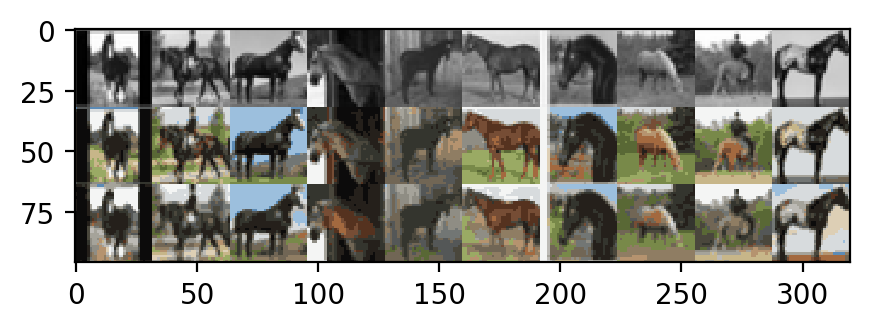
\includegraphics[width=\linewidth]{figures/unet_output_bs_50.png}
		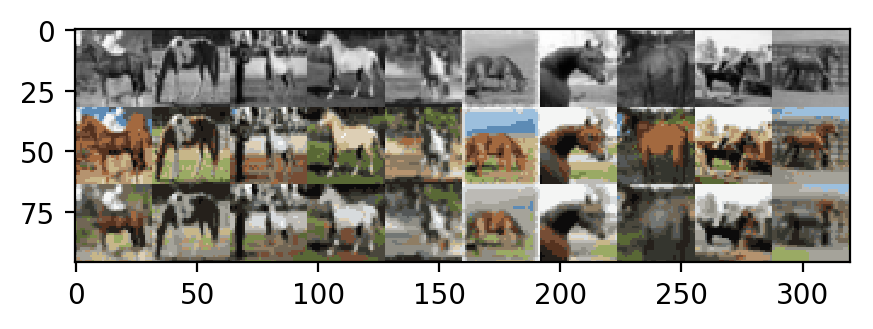
\includegraphics[width=\linewidth]{figures/unet_output_bs_100.png}
		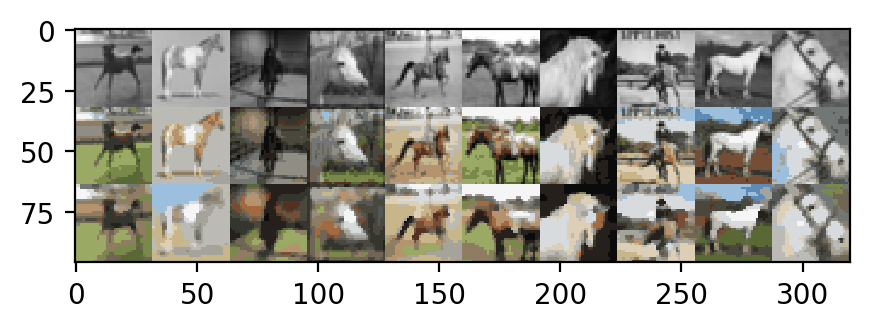
\includegraphics[width=\linewidth]{figures/unet_output_bs_500.png}
		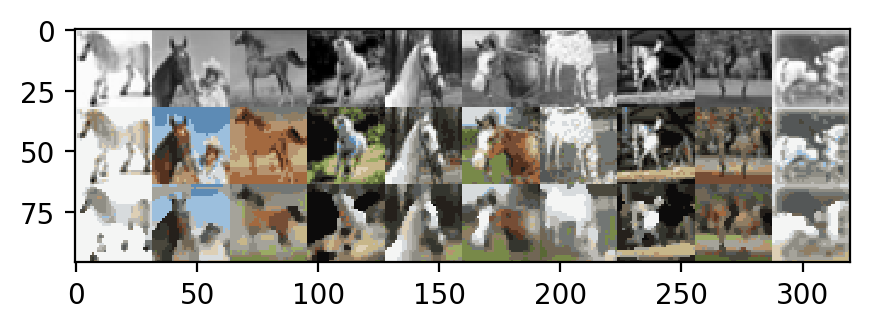
\includegraphics[width=\linewidth]{figures/unet_output_bs_1000.png}
	\end{figure}

	\begin{figure}[H]
		\centering
		\caption{Batchsize=50(left) and 100(right)}
		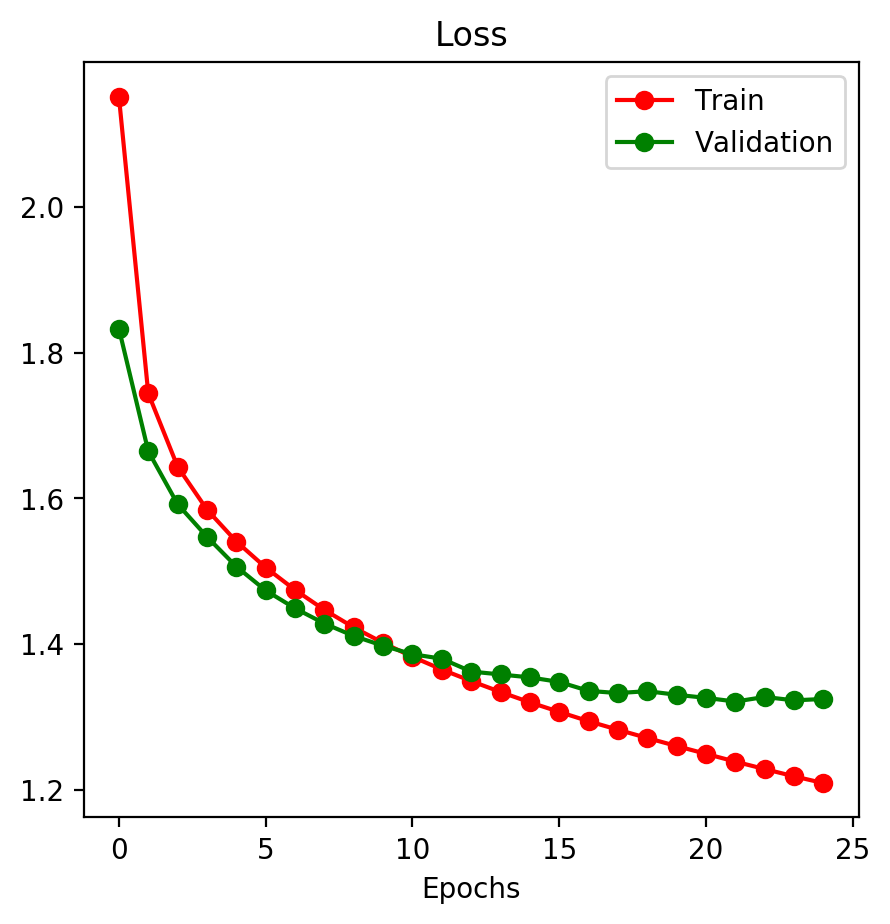
\includegraphics[width=0.45\linewidth]{figures/unet_learning_bs_50.png}
		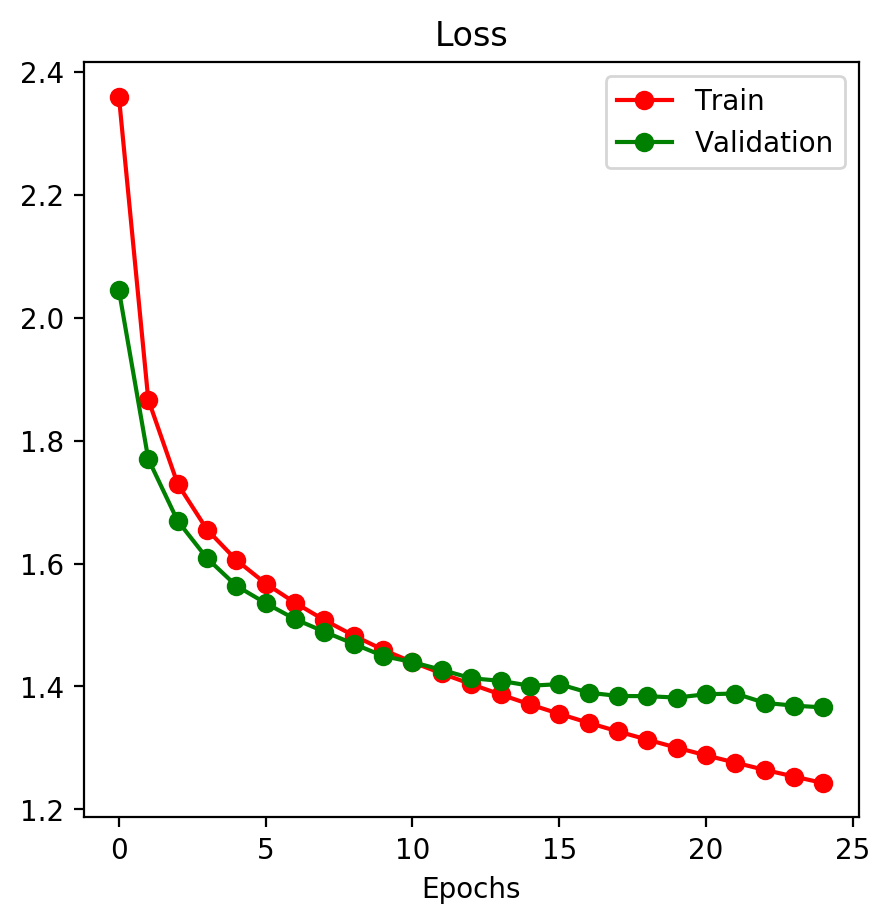
\includegraphics[width=0.45\linewidth]{figures/unet_learning_bs_100.png}
	\end{figure}

	\begin{figure}[H]
		\centering
		\caption{Batchsize=500(left) and 1,000(right)}
		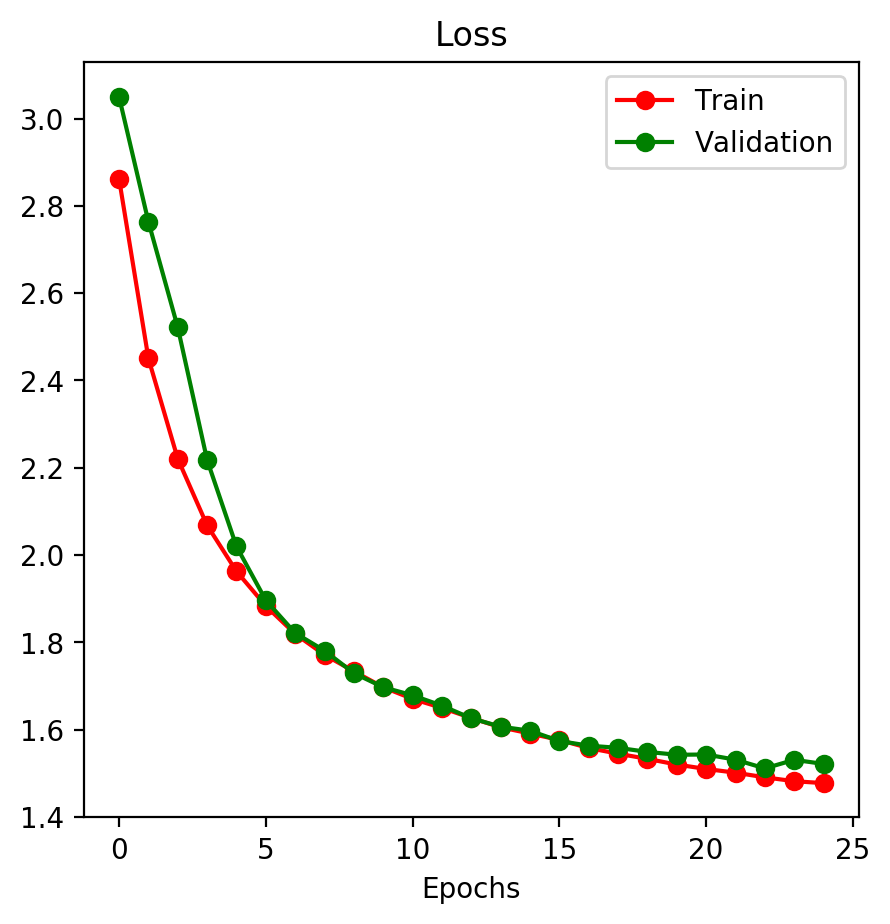
\includegraphics[width=0.45\linewidth]{figures/unet_learning_bs_500.png}
		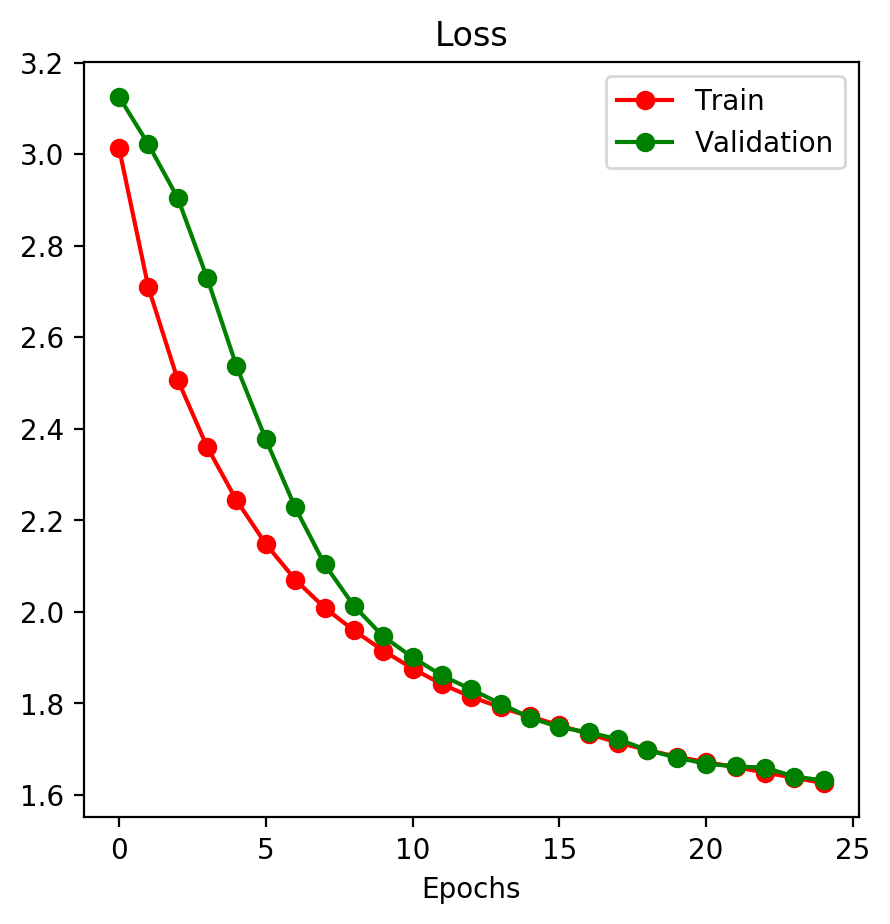
\includegraphics[width=0.45\linewidth]{figures/unet_learning_bs_1000.png}
	\end{figure}
	
	\section{Fine-tune Semantic Segmentation Model}
	\paragraph{Question 1} Implementation:
	\begin{lstlisting}[language=python]
for name, param in model.named_parameters():
    if name.startswith("classifier.4"):
        learned_parameters.append(param)
	\end{lstlisting}
	\paragraph{Question 2} Implementation:
	\begin{lstlisting}[language=python]
model.requires_grad_(False)
model.classifier[4] = nn.Conv2d(
	256, 21, kernel_size=(1, 1), stride=(1, 1)
)
	\end{lstlisting}
	
	\paragraph{Question 3} The visualized predictions:
	\begin{figure}[H]
		\centering
		\caption{Prediction on Training (top) and Validation (bottom) Set}
		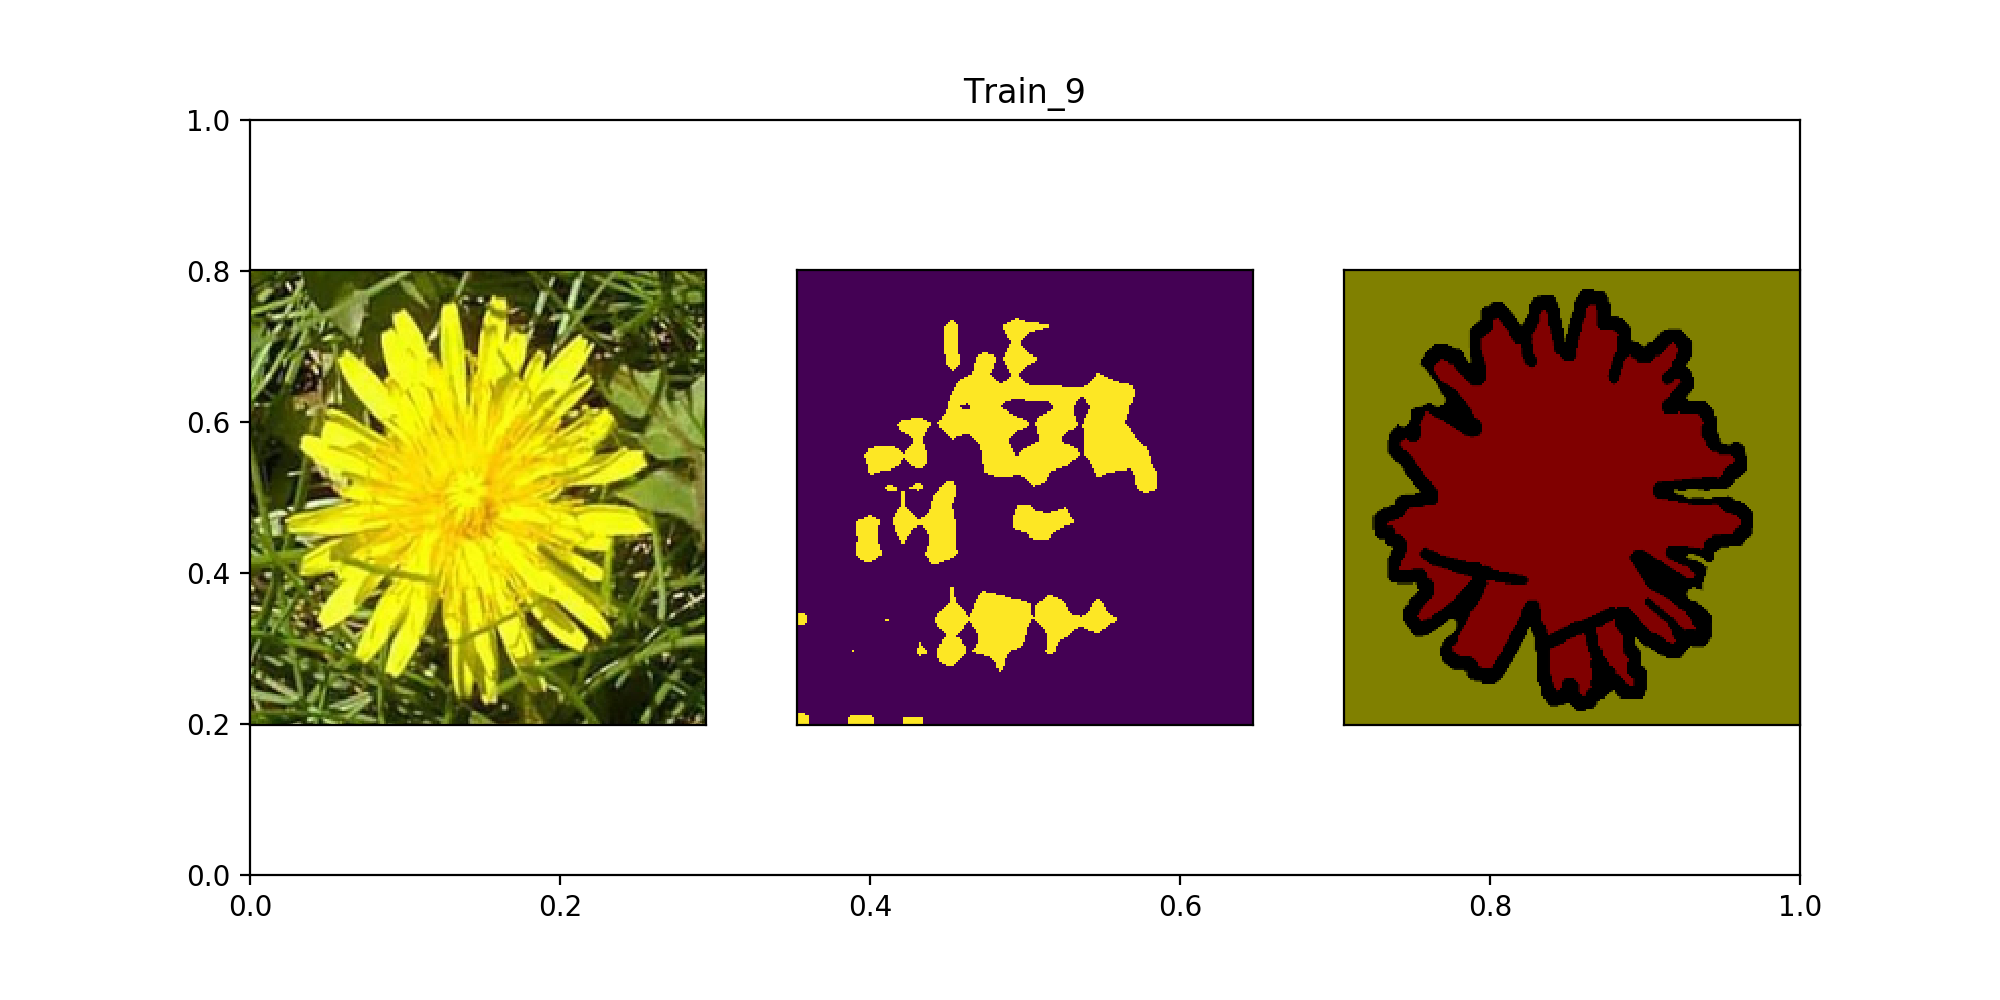
\includegraphics[width=\linewidth]{figures/c3_train_9.png}
		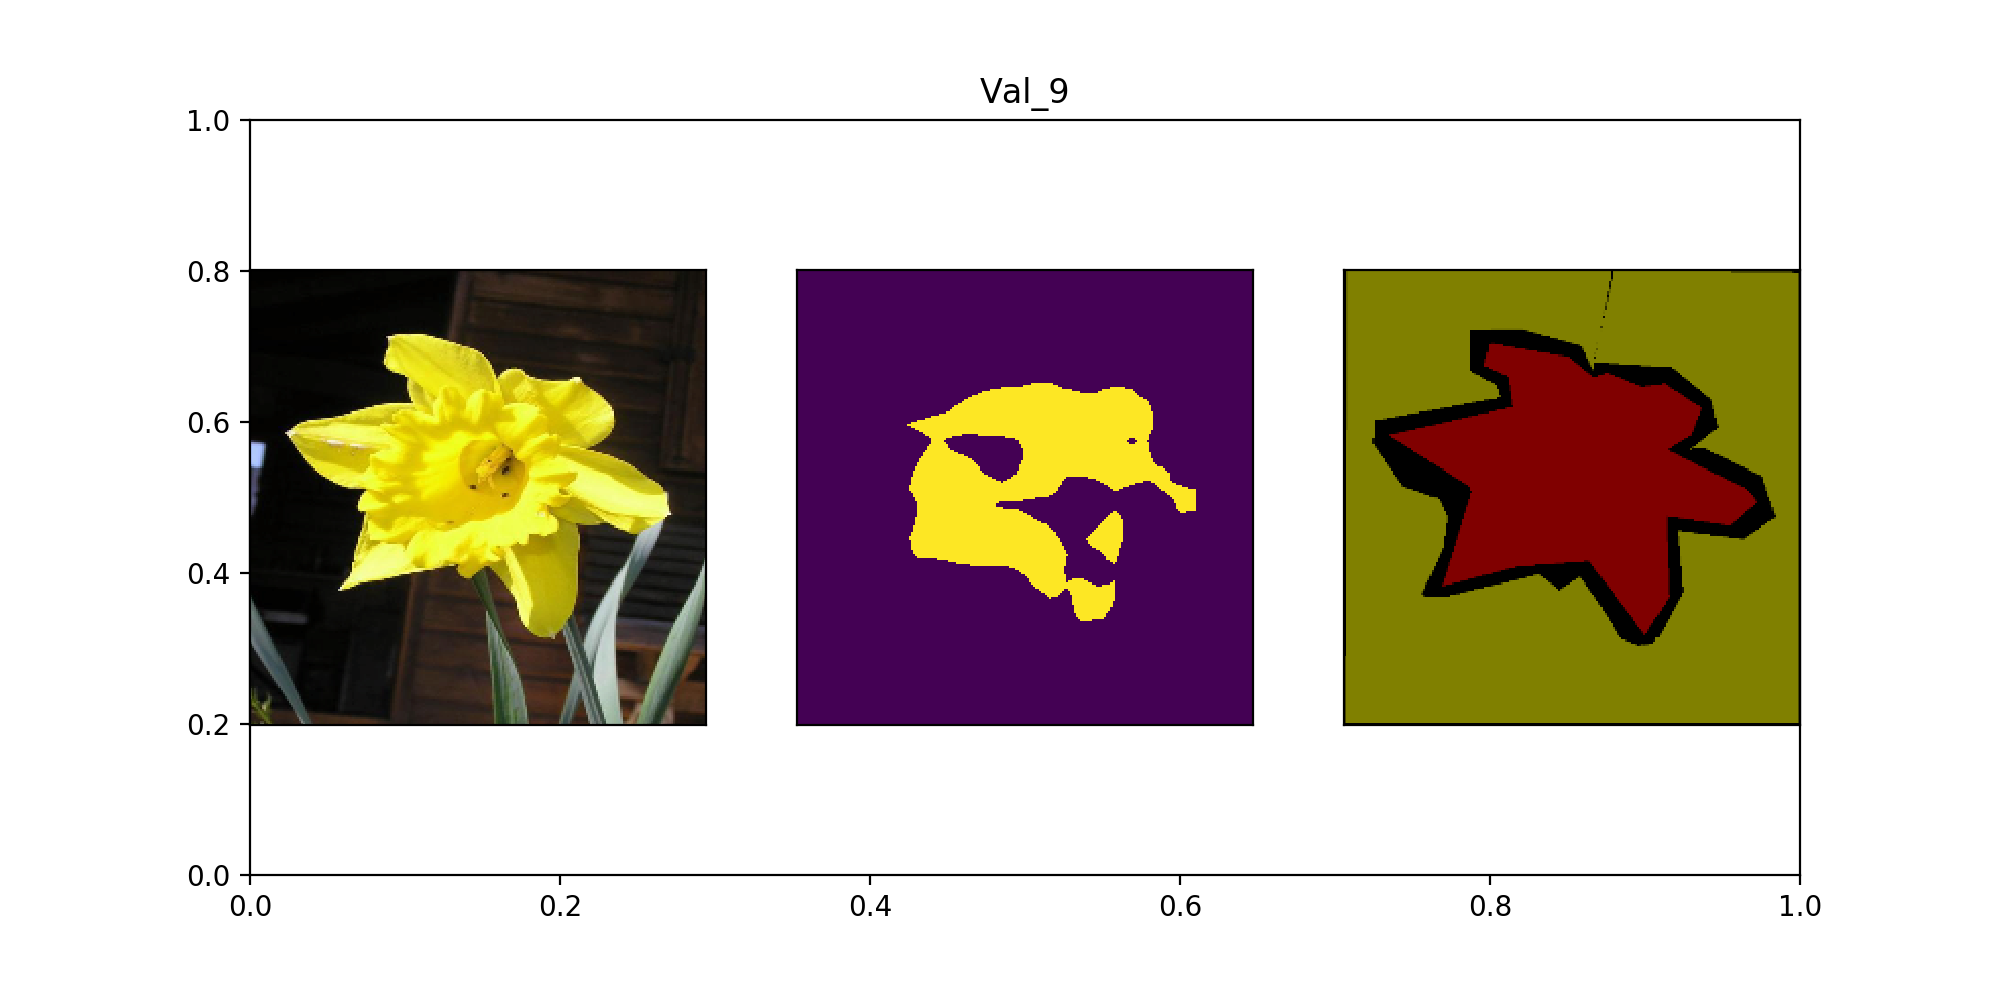
\includegraphics[width=\linewidth]{figures/c3_val_9.png}
	\end{figure}

	\begin{figure}[H]
		\centering
	\end{figure}

	\paragraph{Question 4} The memory required of tuning the entire model involves storing all trainable parameters and the gradient with respect to each trainable parameter. The overall memory complexity of tuning the entire model is in $\mc{O}(n)$, and tuning only one layer is in $\mc{O}(1)$. \\
	The computational complexity of backward propagation is approximately 200\% of the forward passing. Since the number of connections between two consecutive layers is constant, the computational complexity of training $n$ layers is in $\mc{O}(n)$. \\
	Hence, tuning the entire model has computational complexity of $\mc{O}(n)$ while tuning only the last layer costs $\mc{O}(1)$.
	
	\paragraph{Question 5} The number of trainable parameters in each layer within this model only depends on kernel sizes, number of input channels and number of output channels. These numbers are unchanged when the size of input image changes. Therefore, the total number of parameters and memory needed to store the model is unchanged. However, the new dataset with larger images now requires 400\% memory, compared with the original dataset, to be stored.
\end{document}
























